\documentclass[10pt]{article}
\usepackage[polish]{babel}
\usepackage[utf8]{inputenc}
\usepackage[T1]{fontenc}
\usepackage{graphicx}
\usepackage[export]{adjustbox}
\graphicspath{ {./images/} }
\usepackage{hyperref}
\hypersetup{colorlinks=true, linkcolor=blue, filecolor=magenta, urlcolor=cyan,}
\urlstyle{same}
\usepackage{amsmath}
\usepackage{amsfonts}
\usepackage{amssymb}
\usepackage[version=4]{mhchem}
\usepackage{stmaryrd}

\title{PRÓBNY EGZAMIN MATURALNY Z MATEMATYKI }

\author{}
\date{}


\newcommand\Varangle{\mathop{{<\!\!\!\!\!\text{\small)}}\:}\nolimits}

\begin{document}
\maketitle
UZUPEŁNIA ZDAJĄCY\\
Dostosowanie\\
wymagań\\

\includegraphics[max width=\textwidth, center]{2024_11_21_ba65d61981011633d840g-01(1)}

\section*{POZIOM PODSTAWOWY}
MARZEC

Czas pracy: 170 minut\\
Liczba punktów do uzyskania: 50\\
2020 ROK

Instrukcja dla zdającego

\begin{enumerate}
  \item Sprawdź, czy arkusz egzaminacyjny zawiera 20 stron (zadania 1-34).
\end{enumerate}

Ewentualny brak zgłłó przewodniczącemu zespołu nadzorującego egzamin.\\
2. Rozwiązania zadań i odpowiedzi wpisuj w miejscu na to przeznaczonym.\\
3. Odpowiedzi do zadań zamkniętych (1-25) przenieś na kartę odpowiedzi, zaznaczając je w części karty przeznaczonej dla zdającego.\\
4. Zamaluj pola do tego przeznaczone.

Błędne zaznaczenie otocz kółkiem (1) i zaznacz właściwe.\\
5. Pamiętaj, że pominięcie argumentacji lub istotnych obliczeń w rozwiązaniu zadania otwartego (26-34) może spowodować, że za to rozwiązanie nie otrzymasz pełnej liczby punktów.\\
6. Pisz czytelnie i używaj tylko długopisu lub pióra z czarnym tuszem lub atramentem.\\
7. Nie używaj korektora, a błędne zapisy wyraźnie przekreśl.\\
8. Pamiętaj, że zapisy w brudnopisie nie będą oceniane.\\
9. Możesz korzystać z zestawu wzorów matematycznych, cyrkla i linijki oraz kalkulatora prostego.

\section*{Życzymy powodzenia!}
\begin{center}

\includegraphics[max width=\textwidth]{2024_11_21_ba65d61981011633d840g-01}
\end{center}

WYŻSZA SZKOŁA EKONOMII, PRAWA I NAUK MEDYCZNYCH W KIELCACH\\
\href{http://wseip.edu.pl}{wseip.edu.pl}

Prawa autorskie posiada Polska Press Sp. z o.o. Oddział w Kielcach, wydawca Echa Dnia. Kopiowanie w całości lub we fragmentach bez zgody Wydawcy zabronione.

\section*{ZADANIA ZAMKNIĘTE}
W zadaniach od 1. do 25. wybierz i zaznacz na karcie odpowiedzi poprawnq odpowiedź.

\section*{Zadanie 1. (0-1)}
Liczba \(8^{12} \cdot 16^{-7}\) jest równa\\
A. \(\frac{1}{256}\)\\
B. 128\\
C. \(2^{8}\)\\
D. \(\left(\frac{1}{2}\right)^{5}\)

\section*{Zadanie 2. (0-1)}
Wartość wyrażenia \(\log _{3} 30-\log _{3} 5\) jest równa\\
A. 2\\
B. \(\log _{3} 150\)\\
C. \(\log _{3} 25\)\\
D. \(-1+\log _{3} 18\)

\section*{Zadanie 3. (0-1)}
Wartość wyrażenia \(\sqrt[4]{4 \sqrt[3]{4}}\) jest równa\\
A. \(\sqrt[3]{4}\)\\
B. \(\sqrt[3]{2}\)\\
C. \(\sqrt[4]{4}\)\\
D. \(\sqrt[4]{2}\)

\section*{Zadanie 4. (0-1)}
Gdyby cenę towaru A obniżono o \(10 \%\), a cenę towaru B podwyższono o \(8 \%\), to okazałoby się, że ceny te byłyby równe. Wynika stąd, że cena towaru A jest wyższa od ceny towaru B o\\
A. \(18 \%\)\\
B. \(19 \%\)\\
C. \(20 \%\)\\
D. \(22 \%\)

\section*{Zadanie 5. (0-1)}
Wskaż liczbę, która nie należy do zbioru rozwiązań nierówności \(\left(1-x^{2}\right)(3 x-2) \leq 2\).\\
A. -1\\
B. -2\\
C. 0\\
D. 1

\section*{Zadanie 6. (0-1)}
Wartość wyrażenia \((2 a-b)^{2}\) dla \(a=2 \sqrt{7}\) i \(b=\sqrt{175}\) jest równa\\
A. 147\\
B. 49\\
C. \(\sqrt{7}\)\\
D. 7

Próbny egzamin maturalny z matematyki - POZIOM PODSTAWOWY - MARZEC 2020\\
BRUDNOPIS (nie podlega ocenianiu)

\begin{center}
\begin{tabular}{|c|c|c|c|c|c|c|c|c|c|c|c|c|c|c|c|c|c|c|c|c|c|c|c|c|}
\hline
 &  &  &  &  &  &  &  &  &  &  &  &  &  &  &  &  &  &  &  &  &  &  &  &  \\
\hline
 &  &  &  &  &  &  &  &  &  &  &  &  &  &  &  &  &  &  &  &  &  &  &  &  \\
\hline
 &  &  &  &  &  &  &  &  &  &  &  &  &  &  &  &  &  &  &  &  &  &  &  &  \\
\hline
 &  &  &  &  &  &  &  &  &  &  &  &  &  &  &  &  &  &  &  &  &  &  &  &  \\
\hline
 &  &  &  &  &  &  &  &  &  &  &  &  &  &  &  &  &  &  &  &  &  &  &  &  \\
\hline
 &  &  &  &  &  &  &  &  &  &  &  &  &  &  &  &  &  &  &  &  &  &  &  &  \\
\hline
 &  &  &  &  &  &  &  &  &  &  &  &  &  &  &  &  &  &  &  &  &  &  &  &  \\
\hline
 &  &  &  &  &  &  &  &  &  &  &  &  &  &  &  &  &  &  &  &  &  &  &  &  \\
\hline
 &  &  &  &  &  &  &  &  &  &  &  &  &  &  &  &  &  &  &  &  &  &  &  &  \\
\hline
 &  &  &  &  &  &  &  &  &  &  &  &  &  &  &  &  &  &  &  &  &  &  &  &  \\
\hline
 &  &  &  &  &  &  &  &  &  &  &  &  &  &  &  &  &  &  &  &  &  &  &  &  \\
\hline
 &  &  &  &  &  &  &  &  &  &  &  &  &  &  &  &  &  &  &  &  &  &  &  &  \\
\hline
 &  &  &  &  &  &  &  &  &  &  &  &  &  &  &  &  &  &  &  &  &  &  &  &  \\
\hline
 &  &  &  &  &  &  &  &  &  &  &  &  &  &  &  &  &  &  &  &  &  &  &  &  \\
\hline
 &  &  &  &  &  &  &  &  &  &  &  &  &  &  &  &  &  &  &  &  &  &  &  &  \\
\hline
 &  &  &  &  &  &  &  &  &  &  &  &  &  &  &  &  &  &  &  &  &  &  &  &  \\
\hline
 &  &  &  &  &  &  &  &  &  &  &  &  &  &  &  &  &  &  &  &  &  &  &  &  \\
\hline
 &  &  &  &  &  &  &  &  &  &  &  &  &  &  &  &  &  &  &  &  &  &  &  &  \\
\hline
 &  &  &  &  &  &  &  &  &  &  &  &  &  &  &  &  &  &  &  &  &  &  &  &  \\
\hline
 &  &  &  &  &  &  &  &  &  &  &  &  &  &  &  &  &  &  &  &  &  &  &  &  \\
\hline
 &  &  &  &  &  &  &  &  &  &  &  &  &  &  &  &  &  &  &  &  &  &  &  &  \\
\hline
 &  &  &  &  &  &  &  &  &  &  &  &  &  &  &  &  &  &  &  &  &  &  &  &  \\
\hline
 &  &  &  &  &  &  &  &  &  &  &  &  &  &  &  &  &  &  &  &  &  &  &  &  \\
\hline
 &  &  &  &  &  &  &  &  &  &  &  &  &  &  &  &  &  &  &  &  &  &  &  &  \\
\hline
 &  &  &  &  &  &  &  &  &  &  &  &  &  &  &  &  &  &  &  &  &  &  &  &  \\
\hline
 &  &  &  &  &  &  &  &  &  &  &  &  &  &  &  &  &  &  &  &  &  &  &  &  \\
\hline
 &  &  &  &  &  &  &  &  &  &  &  &  &  &  &  &  &  &  &  &  &  &  &  &  \\
\hline
 &  &  &  &  &  &  &  &  &  &  &  &  &  &  &  &  &  &  &  &  &  &  &  &  \\
\hline
 &  &  &  &  &  &  &  &  &  &  &  &  &  &  &  &  &  &  &  &  &  &  &  &  \\
\hline
 &  &  &  &  &  &  &  &  &  &  &  &  &  &  &  &  &  &  &  &  &  &  &  &  \\
\hline
 &  &  &  &  &  &  &  &  &  &  &  &  &  &  &  &  &  &  &  &  &  &  &  &  \\
\hline
 &  &  &  &  &  &  &  &  &  &  &  &  &  &  &  &  &  &  &  &  &  &  &  &  \\
\hline
 &  &  &  &  &  &  &  &  &  &  &  &  &  &  &  &  &  &  &  &  &  &  &  &  \\
\hline
 &  &  &  &  &  &  &  &  &  &  &  &  &  &  &  &  &  &  &  &  &  &  &  &  \\
\hline
 &  &  &  &  &  &  &  &  &  &  &  &  &  &  &  &  &  &  &  &  &  &  &  &  \\
\hline
 &  &  &  &  &  &  &  &  &  &  &  &  &  &  &  &  &  &  &  &  &  &  &  &  \\
\hline
 &  &  &  &  &  &  &  &  &  &  &  &  &  &  &  &  &  &  &  &  &  &  &  &  \\
\hline
 &  &  &  &  &  &  &  &  &  &  &  &  &  &  &  &  &  &  &  &  &  &  &  &  \\
\hline
 &  &  &  &  &  &  &  &  &  &  &  &  &  &  &  &  &  &  &  &  &  &  &  &  \\
\hline
 &  &  &  &  &  &  &  &  &  &  &  &  &  &  &  &  &  &  &  &  &  &  &  &  \\
\hline
 &  &  &  &  &  &  &  &  &  &  &  &  &  &  &  &  &  &  &  &  &  &  &  &  \\
\hline
 &  &  &  &  &  &  &  &  &  &  &  &  &  &  &  &  &  &  &  &  &  &  &  &  \\
\hline
 &  &  &  &  &  &  & - &  &  &  &  &  &  &  &  &  &  & - &  &  &  &  &  &  \\
\hline
 &  &  &  &  &  &  &  &  &  &  &  &  &  &  &  &  &  &  &  &  &  &  &  &  \\
\hline
\end{tabular}
\end{center}

\section*{Zadanie 7. (0-1)}
Jednym z miejsc zerowych funkcji \(f(x)=-2 m x^{2}+2 x-3\) jest \(x=-\frac{1}{2}\). Stąd wynika że\\
A. \(m=0\)\\
B. \(m=-8\)\\
C. \(m=3\)\\
D. \(m=-2\)

\section*{Zadanie 8. (0-1)}
lloczyn wszystkich rzeczywistych rozwiązań równania \(\left(x^{2}+4\right)\left(x^{2}-3\right)(3 x-2)=0\) jest równy\\
A. \(-\frac{4 \sqrt{3}}{3}\)\\
B. 8\\
C. -2\\
D. \(\frac{2 \sqrt{3}}{3}\)

\section*{Poniższy wykres dotyczy zadań 9. i 10.}
Na rysunku przedstawiono wykres funkcji \(y=f(x)\).\\
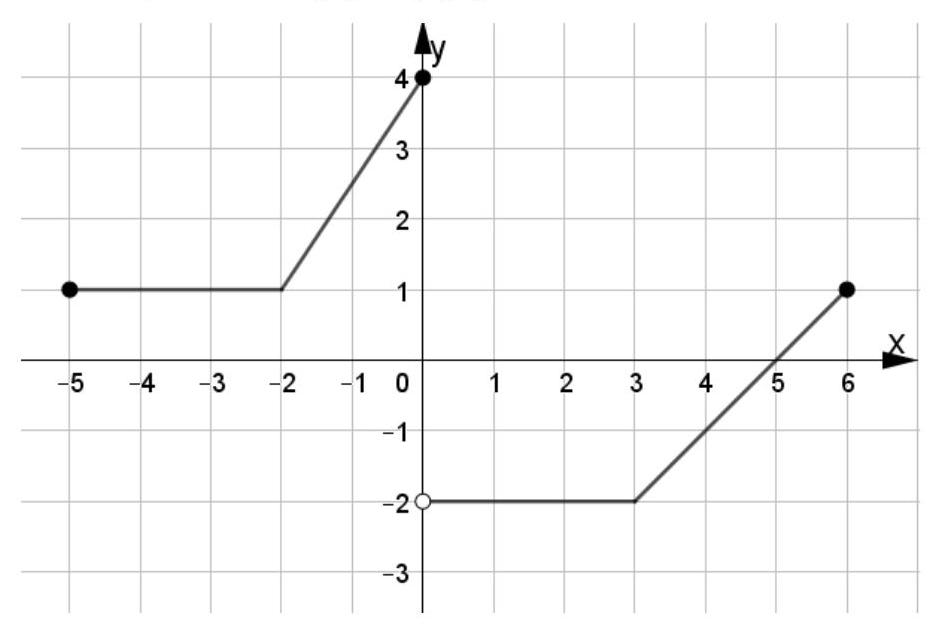
\includegraphics[max width=\textwidth, center]{2024_11_21_ba65d61981011633d840g-04}

\section*{Zadanie 9. (0-1)}
Zbiorem wartości funkcji \(f\) jest\\
A. \(\langle-5 ; 6\rangle\)\\
B. \(\langle-2 ; 4\rangle\)\\
C. \((-2 ; 4\rangle\)\\
D. \((-5 ; 6)\)

\section*{Zadanie 10. (0-1)}
Miejscem zerowym funkcji \(g(x)=f(x)-4\) jest\\
A. 3\\
B. 9\\
C. 1\\
D. 0

\section*{Zadanie 11. (0-1)}
Osią symetrii wykresu funkcji \(f(x)=-3(x-3)(x+5)\) jest prosta o równaniu\\
A. \(x=-1\)\\
B. \(x=1\)\\
C. \(y=-1\)\\
D. \(y=48\)

Próbny egzamin maturalny z matematyki - POZIOM PODSTAWOWY - MARZEC 2020\\
BRUDNOPIS (nie podlega ocenianiu)

\begin{center}
\begin{tabular}{|c|c|c|c|c|c|c|c|c|c|c|c|c|c|c|c|c|c|c|c|c|c|c|c|c|}
\hline
 &  &  &  &  &  &  &  &  &  &  &  &  &  &  &  &  &  &  &  &  &  &  &  &  \\
\hline
 &  &  &  &  &  &  &  &  &  &  &  &  &  &  &  &  &  &  &  &  &  &  &  &  \\
\hline
 &  &  &  &  &  &  &  &  &  &  &  &  &  &  &  &  &  &  &  &  &  &  &  &  \\
\hline
 &  &  &  &  &  &  &  &  &  &  &  &  &  &  &  &  &  &  &  &  &  &  &  &  \\
\hline
 &  &  &  &  &  &  &  &  &  &  &  &  &  &  &  &  &  &  &  &  &  &  &  &  \\
\hline
 &  &  &  &  &  &  &  &  &  &  &  &  &  &  &  &  &  &  &  &  &  &  &  &  \\
\hline
 &  &  &  &  &  &  &  &  &  &  &  &  &  &  &  &  &  &  &  &  &  &  &  &  \\
\hline
 &  &  &  &  &  &  &  &  &  &  &  &  &  &  &  &  &  &  &  &  &  &  &  &  \\
\hline
 &  &  &  &  &  &  &  &  &  &  &  &  &  &  &  &  &  &  &  &  &  &  &  &  \\
\hline
 &  &  &  &  &  &  &  &  &  &  &  &  &  &  &  &  &  &  &  &  &  &  &  &  \\
\hline
 &  &  &  &  &  &  &  &  &  &  &  &  &  &  &  &  &  &  &  &  &  &  &  &  \\
\hline
 &  &  &  &  &  &  &  &  &  &  &  &  &  &  &  &  &  &  &  &  &  &  &  &  \\
\hline
 &  &  &  &  &  &  &  &  &  &  &  &  &  &  &  &  &  &  &  &  &  &  &  &  \\
\hline
 &  &  &  &  &  &  &  &  &  &  &  &  &  &  &  &  &  &  &  &  &  &  &  &  \\
\hline
 &  &  &  &  &  &  &  &  &  &  &  &  &  &  &  &  &  &  &  &  &  &  &  &  \\
\hline
 &  &  &  &  &  &  &  &  &  &  &  &  &  &  &  &  &  &  &  &  &  &  &  &  \\
\hline
 &  &  &  &  &  &  &  &  &  &  &  &  &  &  &  &  &  &  &  &  &  &  &  &  \\
\hline
 &  &  &  &  &  &  &  &  &  &  &  &  &  &  &  &  &  &  &  &  &  &  &  &  \\
\hline
 &  &  &  &  &  &  &  &  &  &  &  &  &  &  &  &  &  &  &  &  &  &  &  &  \\
\hline
 &  &  &  &  &  &  &  &  &  &  &  &  &  &  &  &  &  &  &  &  &  &  &  &  \\
\hline
 &  &  &  &  &  &  &  &  &  &  &  &  &  &  &  &  &  &  &  &  &  &  &  &  \\
\hline
 &  &  &  &  &  &  &  &  &  &  &  &  &  &  &  &  &  &  &  &  &  &  &  &  \\
\hline
 &  &  &  &  &  &  &  &  &  &  &  &  &  &  &  &  &  &  &  &  &  &  &  &  \\
\hline
 &  &  &  &  &  &  &  &  &  &  &  &  &  &  &  &  &  &  &  &  &  &  &  &  \\
\hline
 &  &  &  &  &  &  &  &  &  &  &  &  &  &  &  &  &  &  &  &  &  &  &  &  \\
\hline
 &  &  &  &  &  &  &  &  &  &  &  &  &  &  &  &  &  &  &  &  &  &  &  &  \\
\hline
 &  &  &  &  &  &  &  &  &  &  &  &  &  &  &  &  &  &  &  &  &  &  &  &  \\
\hline
 &  &  &  &  &  &  &  &  &  &  &  &  &  &  &  &  &  &  &  &  &  &  &  &  \\
\hline
 &  &  &  &  &  &  &  &  &  &  &  &  &  &  &  &  &  &  &  &  &  &  &  &  \\
\hline
 &  &  &  &  &  &  &  &  &  &  &  &  &  &  &  &  &  &  &  &  &  &  &  &  \\
\hline
 &  &  &  &  &  &  &  &  &  &  &  &  &  &  &  &  &  &  &  &  &  &  &  &  \\
\hline
 &  &  &  &  &  &  &  &  &  &  &  &  &  &  &  &  &  &  &  &  &  &  &  &  \\
\hline
 &  &  &  &  &  &  &  &  &  &  &  &  &  &  &  &  &  &  &  &  &  &  &  &  \\
\hline
 &  &  &  &  &  &  &  &  &  &  &  &  &  &  &  &  &  &  &  &  &  &  &  &  \\
\hline
 &  &  &  &  &  &  &  &  &  &  &  &  &  &  &  &  &  &  &  &  &  &  &  &  \\
\hline
 &  &  &  &  &  &  &  &  &  &  &  &  &  &  &  &  &  &  &  &  &  &  &  &  \\
\hline
 &  &  &  &  &  &  &  &  &  &  &  &  &  &  &  &  &  &  &  &  &  &  &  &  \\
\hline
 & 
\includegraphics[max width=\textwidth]{2024_11_21_ba65d61981011633d840g-05}
 &  &  &  &  &  &  &  &  &  &  &  &  &  &  &  &  &  &  &  &  &  &  &  \\
\hline
 &  &  &  &  &  &  &  &  &  &  &  &  &  &  &  &  &  &  &  &  &  &  &  &  \\
\hline
 &  &  &  &  &  &  &  &  &  &  &  &  &  &  &  &  &  &  &  &  &  &  &  &  \\
\hline
 &  &  &  &  &  &  &  &  &  &  &  &  &  &  &  &  &  &  &  &  &  &  &  &  \\
\hline
 &  &  &  &  &  &  &  &  &  &  &  &  &  &  &  &  &  &  &  &  &  &  &  &  \\
\hline
 &  &  &  &  &  &  &  &  &  &  &  &  &  &  &  &  &  &  &  &  &  &  &  &  \\
\hline
 &  &  &  &  &  &  &  &  &  &  &  &  &  &  &  &  &  &  &  &  &  &  &  &  \\
\hline
\end{tabular}
\end{center}

\section*{Zadanie 12. (0-1)}
W układzie współrzędnych przedstawiono część wykresu funkcji liniowej \(f(x)=a x+b\).\\
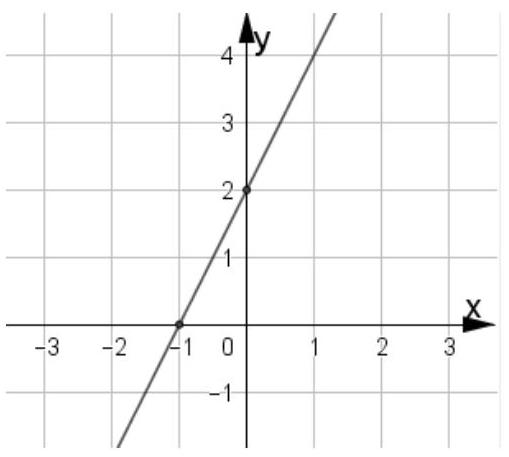
\includegraphics[max width=\textwidth, center]{2024_11_21_ba65d61981011633d840g-06}

Wartość wyrażenia \((2 a-b)\) jest równa\\
A. 4\\
B. 0\\
C. -4\\
D. 2

\section*{Zadanie 13. (0-1)}
W trójkącie równoramiennym \(A B C,|A C|=|B C|=8\) oraz \(|\Varangle C|=120^{\circ}\). Wysokość opuszczona z wierzchołka \(C\) ma długość\\
A. \(\frac{8 \sqrt{3}}{3}\)\\
B. \(2 \sqrt{3}\)\\
C. \(4 \sqrt{3}\)\\
D. 4

\section*{Zadanie 14. (0-1)}
Promień okręgu opisanego na trójkącie równobocznym o boku \(18 \sqrt{3} \mathrm{~cm}\) ma długość\\
A. 18 cm\\
B. 12 cm\\
C. 6 cm\\
D. \(6 \sqrt{3} \mathrm{~cm}\)

\section*{Zadanie 15. (0-1)}
Kąt \(\alpha\) jest ostry i \(\cos \alpha=0,225\). Wtedy \(\operatorname{tg} \alpha\) należy do przedziału\\
A. \((4 ; 5)\)\\
B. \((0 ; 2)\)\\
C. \((2 ; 3)\)\\
D. \((3 ; 4)\)

\section*{Zadanie 16. (0-1)}
Dziesiąty wyraz ciągu arytmetycznego jest równy 32, a różnica tego ciągu jest równa 2 . Wzór ogólny tego ciągu, to\\
A. \(a_{n}=2 n-8\)\\
B. \(a_{n}=2 n+12\)\\
C. \(a_{n}=n+22\)\\
D. \(a_{n}=-2 n+52\)

\section*{Zadanie 17. (0-1)}
Liczby \((2,8,2 x-6)\) w podanej kolejności tworzą trzywyrazowy ciąg geometryczny. Stąd wynika, że\\
A. \(x=18\)\\
B. \(x=32\)\\
C. \(x=12\)\\
D. \(x=19\)

Próbny egzamin maturalny z matematyki - POZIOM PODSTAWOWY - MARZEC 2020\\
BRUDNOPIS (nie podlega ocenianiu)\\

\includegraphics[max width=\textwidth, center]{2024_11_21_ba65d61981011633d840g-07}

\section*{Zadanie 18. (0-1)}
Wykresy funkcji liniowych \(f(x)=m^{3} x+12\) oraz \(g(x)=8 x+3 m-1\) są prostopadłe, gdy\\
A. \(m=-\frac{1}{2}\)\\
B. \(m=\frac{1}{2}\)\\
C. \(m=2\)\\
D. \(m=-2\)

\section*{Zadanie 19. (0-1)}
Prosta \(k\) jest równoległa do prostej o równaniu \(y=\frac{2}{3} x+7\) oraz przechodzi przez punkt \(P=(-3,8)\). Zatem prostą \(k\) opisuje równanie\\
A. \(y=\frac{2}{3} x+6\)\\
B. \(y=-\frac{3}{2} x+3 \frac{1}{2}\)\\
C. \(y=\frac{2}{3} x+10\)\\
D. \(y=\frac{3}{2} x+12 \frac{1}{2}\)

\section*{Zadanie 20. (0-1)}
Cięciwa \(A C\) jest równoległa do średnicy \(D E\) okręgu o środku \(S\) (zobacz rysunek).\\
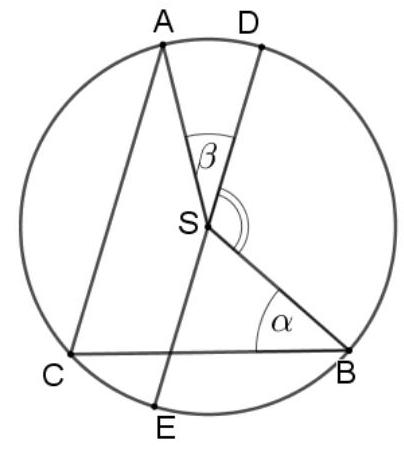
\includegraphics[max width=\textwidth, center]{2024_11_21_ba65d61981011633d840g-08(1)}

Miara kąta wypukłego \(B S D\) jest równa\\
A. \(\alpha+\beta\)\\
B. \(\alpha+2 \beta\)\\
C. \(2 \alpha+\beta\)\\
D. \(2 \alpha-\beta\)

\section*{Zadanie 21. (0-1)}
Wiadomo, że \(\alpha+\beta+\gamma=180^{\circ}\).\\
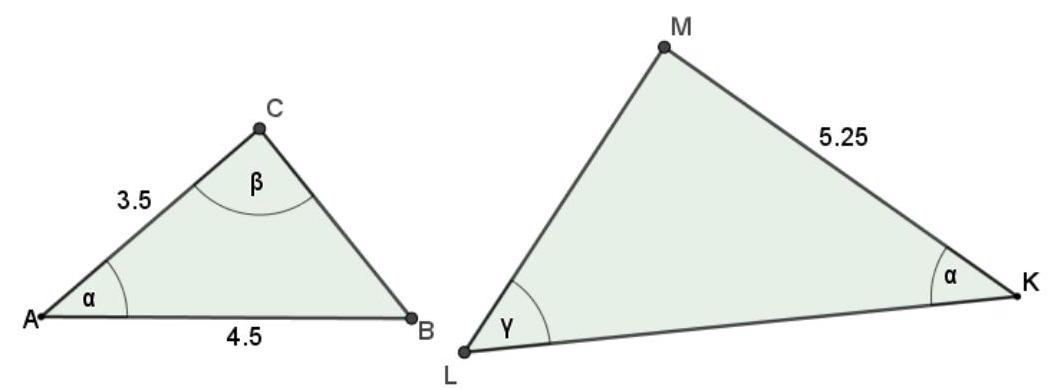
\includegraphics[max width=\textwidth, center]{2024_11_21_ba65d61981011633d840g-08}

Trójkąt \(A B C\) jest podobny do trójkąta \(K L M\) w skali \(k\) równej\\
A. \(\frac{6}{7}\)\\
B. \(\frac{7}{6}\)\\
C. \(\frac{3}{2}\)\\
D. \(\frac{2}{3}\)

Próbny egzamin maturalny z matematyki - POZIOM PODSTAWOWY - MARZEC 2020\\
BRUDNOPIS (nie podlega ocenianiu)

\begin{center}
\begin{tabular}{|c|c|c|c|c|c|c|c|c|c|c|c|c|c|c|c|c|c|c|c|c|c|c|c|c|}
\hline
 &  &  &  &  &  &  &  &  &  &  &  &  &  &  &  &  &  &  &  &  &  &  &  &  \\
\hline
 &  &  &  &  &  &  &  &  &  &  &  &  &  &  &  &  &  &  &  &  &  &  &  &  \\
\hline
 &  &  &  &  &  &  &  &  &  &  &  &  &  &  &  &  &  &  &  &  &  &  &  &  \\
\hline
 &  &  &  &  &  &  &  &  &  &  &  &  &  &  &  &  &  &  &  &  &  &  &  &  \\
\hline
 &  &  &  &  &  &  &  &  &  &  &  &  &  &  &  &  &  &  &  &  &  &  &  &  \\
\hline
 &  &  &  &  &  &  &  &  &  &  &  &  &  &  &  &  &  &  &  &  &  &  &  &  \\
\hline
 &  &  &  &  &  &  &  &  &  &  &  &  &  &  &  &  &  &  &  &  &  &  &  &  \\
\hline
 &  &  &  &  &  &  &  &  &  &  &  &  &  &  &  &  &  &  &  &  &  &  &  &  \\
\hline
 &  &  &  &  &  &  &  &  &  &  &  &  &  &  &  &  &  &  &  &  &  &  &  &  \\
\hline
 &  &  &  &  &  &  &  &  &  &  &  &  &  &  &  &  &  &  &  &  &  &  &  &  \\
\hline
 &  &  &  &  &  &  &  &  &  &  &  &  &  &  &  &  &  &  &  &  &  &  &  &  \\
\hline
 &  &  &  &  &  &  &  &  &  &  &  &  &  &  &  &  &  &  &  &  &  &  &  &  \\
\hline
 &  &  &  &  &  &  &  &  &  &  &  &  &  &  &  &  &  &  &  &  &  &  &  &  \\
\hline
 &  &  &  &  &  &  &  &  &  &  &  &  &  &  &  &  &  &  &  &  &  &  &  &  \\
\hline
 &  &  &  &  &  &  &  &  &  &  &  &  &  &  &  &  &  &  &  &  &  &  &  &  \\
\hline
 &  &  &  &  &  &  &  &  &  &  &  &  &  &  &  &  &  &  &  &  &  &  &  &  \\
\hline
 &  &  &  &  &  &  &  &  &  &  &  &  &  &  &  &  &  &  &  &  &  &  &  &  \\
\hline
 &  &  &  &  &  &  &  &  &  &  &  &  &  &  &  &  &  &  &  &  &  &  &  &  \\
\hline
 &  &  &  &  &  &  &  &  &  &  &  &  &  &  &  &  &  &  &  &  &  &  &  &  \\
\hline
 &  &  &  &  &  &  &  &  &  &  &  &  &  &  &  &  &  &  &  &  &  &  &  &  \\
\hline
 &  &  &  &  &  &  &  &  &  &  &  &  &  &  &  &  &  &  &  &  &  &  &  &  \\
\hline
 &  &  &  &  &  &  &  &  &  &  &  &  &  &  &  &  &  &  &  &  &  &  &  &  \\
\hline
 &  &  &  &  &  &  &  &  &  &  &  &  &  &  &  &  &  &  &  &  &  &  &  &  \\
\hline
 &  &  &  &  &  &  &  &  &  &  &  &  &  &  &  &  &  &  &  &  &  &  &  &  \\
\hline
 &  &  &  &  &  &  &  &  &  &  &  &  &  &  &  &  &  &  &  &  &  &  &  &  \\
\hline
 &  &  &  &  &  &  &  &  &  &  &  &  &  &  &  &  &  &  &  &  &  &  &  &  \\
\hline
 &  &  &  &  &  &  &  &  &  &  &  &  &  &  &  &  &  &  &  &  &  &  &  &  \\
\hline
 &  &  &  &  &  &  &  &  &  &  &  &  &  &  &  &  &  &  &  &  &  &  &  &  \\
\hline
 &  &  &  &  &  &  &  &  &  &  &  &  &  &  &  &  &  &  &  &  &  &  &  &  \\
\hline
 &  &  &  &  &  &  &  &  &  &  &  &  &  &  &  &  &  &  &  &  &  &  &  &  \\
\hline
 &  &  &  &  &  &  &  &  &  &  &  &  &  &  &  &  &  &  &  &  &  &  &  &  \\
\hline
 &  &  &  &  &  &  &  &  &  &  &  &  &  &  &  &  &  &  &  &  &  &  &  &  \\
\hline
 &  &  &  &  &  &  &  &  &  &  &  &  &  &  &  &  &  &  &  &  &  &  &  &  \\
\hline
 &  &  &  &  &  &  &  &  &  &  &  &  &  &  &  &  &  &  &  &  &  &  &  &  \\
\hline
 &  &  &  &  &  &  &  &  &  &  &  &  &  &  &  &  &  &  &  &  &  &  &  &  \\
\hline
 &  &  &  &  &  &  &  &  &  &  &  &  &  &  &  &  &  &  &  &  &  &  &  &  \\
\hline
 &  &  &  &  &  &  &  &  &  &  &  &  &  &  &  &  &  &  &  &  &  &  &  &  \\
\hline
 & 
\includegraphics[max width=\textwidth]{2024_11_21_ba65d61981011633d840g-09}
 &  &  &  &  &  &  &  &  &  &  &  &  &  &  &  &  &  &  &  &  &  &  &  \\
\hline
 &  &  &  &  &  &  &  &  &  &  &  &  &  &  &  &  &  &  &  &  &  &  &  &  \\
\hline
 &  &  &  &  &  &  &  &  &  &  &  &  &  &  &  &  &  &  &  &  &  &  &  &  \\
\hline
 &  &  &  &  &  &  &  &  &  &  &  &  &  &  &  &  &  &  &  &  &  &  &  &  \\
\hline
 &  &  &  &  &  &  &  &  &  &  &  &  &  &  &  &  &  &  &  &  &  &  &  &  \\
\hline
 &  &  &  &  &  &  &  &  &  &  &  &  &  &  &  &  &  &  &  &  &  &  &  &  \\
\hline
 &  &  &  &  &  &  &  &  &  &  &  &  &  &  &  &  &  &  &  &  &  &  &  &  \\
\hline
\end{tabular}
\end{center}

Próbny egzamin maturalny z matematyki - POZIOM PODSTAWOWY - MARZEC 2020

\section*{Zadanie 22. (0-1)}
Suma długości wszystkich krawędzi sześcianu jest równa 84 cm . Pole powierzchni całkowitej tej bryły jest równe\\
A. \(294 \mathrm{~cm}^{2}\)\\
B. \(49 \mathrm{~cm}^{2}\)\\
C. \(343 \mathrm{~cm}^{2}\)\\
D. \(1176 \mathrm{~cm}^{2}\)

\section*{Zadanie 23. (0-1)}
Liczb pięciocyfrowych parzystych lub podzielnych przez 5, w zapisie których występują wszystkie cyfry należące do zbioru \(\{1,2,3,4,5\}\) jest\\
A. \(1 \cdot 2 \cdot 3 \cdot 4\)\\
B. \(3 \cdot 4 \cdot 3 \cdot 2\)\\
C. \(2 \cdot 3 \cdot 4 \cdot 5\)\\
D. \(1 \cdot 2 \cdot 3 \cdot 3\)

\section*{Zadanie 24. (0-1)}
Sprzedawca zakupił w hurtowni 80 kg cukierków: 20 kg w cenie15 zł za kilogram oraz 60 kg w cenie 10 zł za kilogram. Zmieszał wszystkie i w swoim sklepie sprzedawał je w cenie 13 zł za kilogram. Zysk sprzedawcy (nie licząc amortyzacji i podatków) jaki uzyska sprzedając 10 kg cukierków jest równy\\
A. \(15 \mathrm{zł}\)\\
B. \(17,5 \mathrm{zł}\)\\
C. 5 z\\
D. 22,5 z

\section*{Zadanie 25. (0-1)}
Ze zbioru liczb naturalnych dwucyfrowych mniejszych od 20 losujemy jedną liczbę. Prawdopodobieństwo wylosowania liczby złożonej jest równe\\
A. \(\frac{6}{10}\)\\
B. \(\frac{5}{10}\)\\
C. \(\frac{6}{9}\)\\
D. \(\frac{5}{9}\)

BRUDNOPIS (nie podlega ocenie)\\

\includegraphics[max width=\textwidth, center]{2024_11_21_ba65d61981011633d840g-10}

\section*{ZADANIA OTWARTE}
Rozwiqzania zadań o numerach od 26. do 34. należy zapisać w wyznaczonych miejscach pod treściq zadania. Zadanie 26. (0-2)\\
Rozwiąż nierówność \(-x^{2}+2 x \leq(x-2)(x-1)\).\\

\includegraphics[max width=\textwidth, center]{2024_11_21_ba65d61981011633d840g-11(1)}

Odpowiedź

\section*{Zadanie 27. (0-2)}
Rozwiąż równanie \(\frac{x^{2}+3 x-4}{2 x-2}=-3\).\\

\includegraphics[max width=\textwidth, center]{2024_11_21_ba65d61981011633d840g-11}

Odpowiedź \(\qquad\)

\section*{Zadanie 28. (0-2)}
Uzasadnij, że dla dowolnych dodatnich liczb rzeczywistych \(x\) i \(y\) spełniona jest nierówność

\[
\frac{2 x^{2}+2 y^{2}+1}{x+y} \geq 2
\]

\begin{center}

\includegraphics[max width=\textwidth]{2024_11_21_ba65d61981011633d840g-12}
\end{center}

\section*{Zadanie 29. (0-2)}
Dany jest trójkąt prostokątny \(\mathrm{ABC}, \mathrm{w}\) którym \(|\Varangle C|=90^{\circ}\). Poprowadzono dwie proste równoległe do przyprostokątnej AC dzielące trójkąt \(A B C\) na trzy figury o równych polach (zobacz rysunek).\\
Uzasadnij, że \(\frac{|\mathrm{FG}|}{|\mathrm{DE}|}=\sqrt{2}\).\\
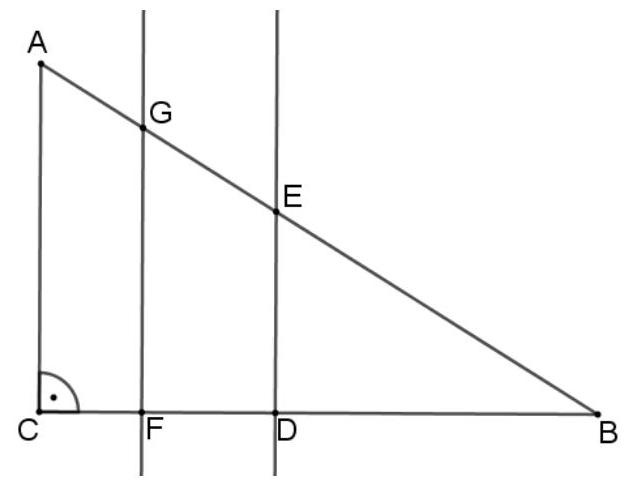
\includegraphics[max width=\textwidth, center]{2024_11_21_ba65d61981011633d840g-13}\\

\includegraphics[max width=\textwidth, center]{2024_11_21_ba65d61981011633d840g-13(1)}

\section*{Zadanie 30. (0-2)}
Dana jest funkcja \(f(x)=-3 x+11\), której dziedziną jest zbiór \(D_{f}=\{0,1,2,3,4,5,6,7\}\). Spośród wszystkich punktów należących do wykresu tej funkcji wybrano jeden. Oblicz prawdopodobieństwo wylosowania punktu, którego suma współrzędnych jest liczbą pierwszą.

\begin{center}
\begin{tabular}{|c|c|c|c|c|c|c|c|c|c|c|c|c|c|c|c|c|c|c|c|c|c|c|c|c|c|c|c|}
\hline
 &  &  &  &  &  &  &  &  &  &  &  &  &  &  &  &  &  &  &  &  &  &  &  &  &  &  &  \\
\hline
 &  &  &  &  &  &  &  &  &  &  &  &  &  &  &  &  &  &  &  &  &  &  &  &  &  &  &  \\
\hline
 &  &  &  &  &  &  &  &  &  &  &  &  &  &  &  &  &  &  &  &  &  &  &  &  &  &  &  \\
\hline
 &  &  &  &  &  &  &  &  &  &  &  &  &  &  &  &  &  &  &  &  &  &  &  &  &  &  &  \\
\hline
 &  &  &  &  &  &  &  &  &  &  &  &  &  &  &  &  &  &  &  &  &  &  &  &  &  &  &  \\
\hline
 &  &  &  &  &  &  &  &  &  &  &  &  &  &  &  &  &  &  &  &  &  &  &  &  &  &  &  \\
\hline
 &  &  &  &  &  &  &  &  &  &  &  &  &  &  &  &  &  &  &  &  &  &  &  &  &  &  &  \\
\hline
 &  &  &  &  &  &  &  &  &  &  &  &  &  &  &  &  &  &  &  &  &  &  &  &  &  &  &  \\
\hline
 &  &  &  &  &  &  &  &  &  &  &  &  &  &  &  &  &  &  &  &  &  &  &  &  &  &  &  \\
\hline
 &  &  &  &  &  &  &  &  &  &  &  &  &  &  &  &  &  &  &  &  &  &  &  &  &  &  &  \\
\hline
 &  &  &  &  &  &  &  &  &  &  &  &  &  &  &  &  &  &  &  &  &  &  &  &  &  &  &  \\
\hline
 &  &  &  &  &  &  &  &  &  &  &  &  &  &  &  &  &  &  &  &  &  &  &  &  &  &  &  \\
\hline
 &  &  &  &  &  &  &  &  &  &  &  &  &  &  &  &  &  &  &  &  &  &  &  &  &  &  &  \\
\hline
 &  &  &  &  &  &  &  &  &  &  &  &  &  &  &  &  &  &  &  &  &  &  &  &  &  &  &  \\
\hline
 &  &  &  &  &  &  &  &  &  &  &  &  &  &  &  &  &  &  &  &  &  &  &  &  &  &  &  \\
\hline
 &  &  &  &  &  &  &  &  &  &  &  &  &  &  &  &  &  &  &  &  &  &  &  &  &  &  &  \\
\hline
 &  &  &  &  &  &  &  &  &  &  &  &  &  &  &  &  &  &  &  &  &  &  &  &  &  &  &  \\
\hline
 &  &  &  &  &  &  &  &  &  &  &  &  &  &  &  &  &  &  &  &  &  &  &  &  &  &  &  \\
\hline
 &  &  &  &  &  &  &  &  &  &  &  &  &  &  &  &  &  &  &  &  &  &  &  &  &  &  &  \\
\hline
 &  &  &  &  &  &  &  &  &  &  &  &  &  &  &  &  &  &  &  &  &  &  &  &  &  &  &  \\
\hline
 & \(\square\) &  &  &  &  &  &  &  &  &  &  &  &  &  &  &  &  &  &  &  &  &  &  &  &  &  &  \\
\hline
 &  &  &  &  &  &  &  &  &  &  &  &  &  &  &  &  &  &  &  &  &  &  &  &  &  &  &  \\
\hline
 &  &  &  &  &  &  &  &  &  &  &  &  &  &  &  &  &  &  &  &  &  &  &  &  &  &  &  \\
\hline
 &  &  &  &  &  &  &  &  &  &  &  &  &  &  &  &  &  &  &  &  &  &  &  &  &  &  &  \\
\hline
 & \textbackslash  &  &  &  &  &  &  &  &  &  &  &  &  &  &  &  &  &  &  &  &  &  &  &  &  &  &  \\
\hline
 & \textbackslash  &  &  &  &  &  &  &  &  &  &  &  &  &  &  &  &  &  &  &  &  &  &  &  &  &  &  \\
\hline
 & - &  &  &  &  &  &  &  &  &  &  &  &  &  &  &  &  &  &  &  &  &  &  &  &  &  &  \\
\hline
 & \textbackslash  &  &  &  &  &  &  &  &  &  &  &  &  &  &  &  &  &  &  &  &  &  &  &  &  &  &  \\
\hline
 & , &  &  &  &  &  &  &  &  &  &  &  &  &  &  &  &  &  &  &  &  &  &  &  &  &  &  \\
\hline
 & 
\includegraphics[max width=\textwidth]{2024_11_21_ba65d61981011633d840g-14}
 &  &  &  &  &  &  &  &  &  &  &  &  &  &  &  &  &  &  &  &  &  &  &  &  &  &  \\
\hline
 &  &  &  &  &  &  &  &  &  &  &  &  &  &  &  &  &  &  &  &  &  &  &  &  &  &  &  \\
\hline
 & \textbackslash  &  &  &  &  &  &  &  &  &  &  &  &  &  &  &  &  &  &  &  &  &  &  &  &  &  &  \\
\hline
 & - &  &  &  &  &  &  &  &  &  &  &  &  &  &  &  &  &  &  &  &  &  &  &  &  &  &  \\
\hline
 &  &  &  &  &  &  &  &  &  &  &  &  &  &  &  &  &  &  &  &  &  &  &  &  &  &  &  \\
\hline
 &  &  &  &  &  &  &  &  &  &  &  &  &  &  &  &  &  &  &  &  &  &  &  &  &  &  &  \\
\hline
 &  &  &  &  &  &  &  &  &  &  &  &  &  &  &  &  &  &  &  &  &  &  &  &  &  &  &  \\
\hline
 &  &  &  &  &  &  &  &  &  &  &  &  &  &  &  &  &  &  &  &  &  &  &  &  &  &  &  \\
\hline
\end{tabular}
\end{center}

\(\qquad\)

\section*{Zadanie 31. (0-2)}
Miary kolejnych kątów wewnętrznych czworokąta tworzą ciąg arytmetyczny o różnicy \(13^{\circ}\). Wyznacz miary kątów tego czworokąta.\\

\includegraphics[max width=\textwidth, center]{2024_11_21_ba65d61981011633d840g-15}

Odpowiedź \(\qquad\)

\section*{Zadanie 32. (0-5)}
Punkt \(A=(-5,-8)\) należy do wykresu funkcji kwadratowej \(f(x)=a x^{2}+b x-3\), a zbiór \((-\infty ;-2\rangle\) jest maksymalnym przedziałem, w którym funkcja ta jest rosnąca. Wyznacz wartości współczynników \(a\) i \(b\) oraz najmniejszą i największą wartość funkcji w przedziale \(\left\langle-3 ;-\frac{1}{2}\right\rangle\).\\

\includegraphics[max width=\textwidth, center]{2024_11_21_ba65d61981011633d840g-16}

\section*{Zadanie 33. (0-4)}
Punkty \(A=\left(-3 \frac{1}{2},-6\right), B=\left(7,1 \frac{1}{2}\right)\) oraz \(C=(1,4)\) są kolejnymi wierzchołkami równoległoboku \(A B C D\). Wyznacz współrzędne punktu \(D\) oraz współrzędne punktu \(E, \mathrm{w}\) którym bok \(C D\) przecina oś odciętych (oś OX) układu współrzędnych.\\

\includegraphics[max width=\textwidth, center]{2024_11_21_ba65d61981011633d840g-17}\\
\(\qquad\)

\section*{Zadanie 34. (0-4)}
Podstawą ostrosłupa prawidłowego trójkątnego \(A B C S\) jest trójkąt \(A B C\). Wysokość \(S D\) ma długość 12 i tworzy z krawędzią boczną kąt, którego tangens jest równy \(\frac{1}{2}\). Oblicz pole powierzchni całkowitej tego ostrosłupa.\\

\includegraphics[max width=\textwidth, center]{2024_11_21_ba65d61981011633d840g-18}

Próbny egzamin maturalny z matematyki - POZIOM PODSTAWOWY - MARZEC 2020

BRUDNOPIS (nie podlega ocenie)

\begin{center}
\begin{tabular}{|c|c|c|c|c|c|c|c|c|c|c|c|c|c|c|c|c|c|c|c|c|c|c|c|c|c|}
\hline
 &  &  &  &  &  &  &  &  &  &  &  &  &  &  &  &  &  &  &  &  &  &  &  &  &  \\
\hline
 &  &  &  &  &  &  &  &  &  &  &  &  &  &  &  &  &  &  &  &  &  &  &  &  &  \\
\hline
 &  &  &  &  &  &  &  &  &  &  &  &  &  &  &  &  &  &  &  &  &  &  &  &  &  \\
\hline
 &  &  &  &  &  &  &  &  &  &  &  &  &  &  &  &  &  &  &  &  &  &  &  &  &  \\
\hline
 &  &  &  &  &  &  &  &  &  &  &  &  &  &  &  &  &  &  &  &  &  &  &  &  &  \\
\hline
 &  &  &  &  &  &  &  &  &  &  &  &  &  &  &  &  &  &  &  &  &  &  &  &  &  \\
\hline
 &  &  &  &  &  &  &  &  &  &  &  &  &  &  &  &  &  &  &  &  &  &  &  &  &  \\
\hline
 &  &  &  &  &  &  &  &  &  &  &  &  &  &  &  &  &  &  &  &  &  &  &  &  &  \\
\hline
 &  &  &  &  &  &  &  &  &  &  &  &  &  &  &  &  &  &  &  &  &  &  &  &  &  \\
\hline
 &  &  &  &  &  &  &  &  &  &  &  &  &  &  &  &  &  &  &  &  &  &  &  &  &  \\
\hline
 &  &  &  &  &  &  &  &  &  &  &  &  &  &  &  &  &  &  &  &  &  &  &  &  &  \\
\hline
 &  &  &  &  &  &  &  &  &  &  &  &  &  &  &  &  &  &  &  &  &  &  &  &  &  \\
\hline
 &  &  &  &  &  &  &  &  &  &  &  &  &  &  &  &  &  &  &  &  &  &  &  &  &  \\
\hline
 &  &  &  &  &  &  &  &  &  &  &  &  &  &  &  &  &  &  &  &  &  &  &  &  &  \\
\hline
 &  &  &  &  &  &  &  &  &  &  &  &  &  &  &  &  &  &  &  &  &  &  &  &  &  \\
\hline
 &  &  &  &  &  &  &  &  &  &  &  &  &  &  &  &  &  &  &  &  &  &  &  &  &  \\
\hline
 &  &  &  &  &  &  &  &  &  &  &  &  &  &  &  &  &  &  &  &  &  &  &  &  &  \\
\hline
 &  &  &  &  &  &  &  &  &  &  &  &  &  &  &  &  &  &  &  &  &  &  &  &  &  \\
\hline
 &  &  &  &  &  &  &  &  &  &  &  &  &  &  &  &  &  &  &  &  &  &  &  &  &  \\
\hline
 &  &  &  &  &  &  &  &  &  &  &  &  &  &  &  &  &  &  &  &  &  &  &  &  &  \\
\hline
 &  &  &  &  &  &  &  &  &  &  &  &  &  &  &  &  &  &  &  &  &  &  &  &  &  \\
\hline
 &  &  &  &  &  &  &  &  &  &  &  &  &  &  &  &  &  &  &  &  &  &  &  &  &  \\
\hline
 &  &  &  &  &  &  &  &  &  &  &  &  &  &  &  &  &  &  &  &  &  &  &  &  &  \\
\hline
 &  &  &  &  &  &  &  &  &  &  &  &  &  &  &  &  &  &  &  &  &  &  &  &  &  \\
\hline
 &  &  &  &  &  &  &  &  &  &  &  &  &  &  &  &  &  &  &  &  &  &  &  &  &  \\
\hline
 &  &  &  &  &  &  &  &  &  &  &  &  &  &  &  &  &  &  &  &  &  &  &  &  &  \\
\hline
 &  &  &  &  &  &  &  &  &  &  &  &  &  &  &  &  &  &  &  &  &  &  &  &  &  \\
\hline
 &  &  &  &  &  &  &  &  &  &  &  &  &  &  &  &  &  &  &  &  &  &  &  &  &  \\
\hline
 &  &  &  &  &  &  &  &  &  &  &  &  &  &  &  &  &  &  &  &  &  &  &  &  &  \\
\hline
 &  &  &  &  &  &  &  &  &  &  &  &  &  &  &  &  &  &  &  &  &  &  &  &  &  \\
\hline
 &  &  &  &  &  &  &  &  &  &  &  &  &  &  &  &  &  &  &  &  &  &  &  &  &  \\
\hline
 &  &  &  &  &  &  &  &  &  &  &  &  &  &  &  &  &  &  &  &  &  &  &  &  &  \\
\hline
 &  &  &  &  &  &  &  &  &  &  &  &  &  &  &  &  &  &  &  &  &  &  &  &  &  \\
\hline
 &  &  &  &  &  &  &  &  &  &  &  &  &  &  &  &  &  &  &  &  &  &  &  &  &  \\
\hline
 &  &  &  &  &  &  &  &  &  &  &  &  &  &  &  &  &  &  &  &  &  &  &  &  &  \\
\hline
 &  &  &  &  &  &  &  &  &  &  &  &  &  &  &  &  &  &  &  &  &  &  &  &  &  \\
\hline
 &  &  &  &  &  &  &  &  &  &  &  &  &  &  &  &  &  &  &  &  &  &  &  &  &  \\
\hline
 &  &  &  &  &  &  &  &  &  &  &  &  &  &  &  &  &  &  &  &  &  &  &  &  &  \\
\hline
 &  &  &  &  &  &  &  &  &  &  &  &  &  &  &  &  &  &  &  &  &  &  &  &  &  \\
\hline
 &  &  &  &  &  &  &  &  &  &  &  &  &  &  &  &  &  &  &  &  &  &  &  &  &  \\
\hline
 &  &  &  &  &  &  &  &  &  &  &  &  &  &  &  &  &  &  &  &  &  &  &  &  &  \\
\hline
 &  &  &  &  &  &  &  &  &  &  &  &  &  &  &  &  &  &  &  &  &  &  &  &  &  \\
\hline
 &  &  &  &  &  &  &  &  &  &  &  &  &  &  &  &  &  &  &  &  &  &  &  &  &  \\
\hline
 &  &  &  &  &  &  &  &  &  &  &  &  &  &  &  &  &  &  &  &  &  &  &  &  &  \\
\hline
\end{tabular}
\end{center}

\section*{KARTA ODPOWIEDZI}
\begin{center}
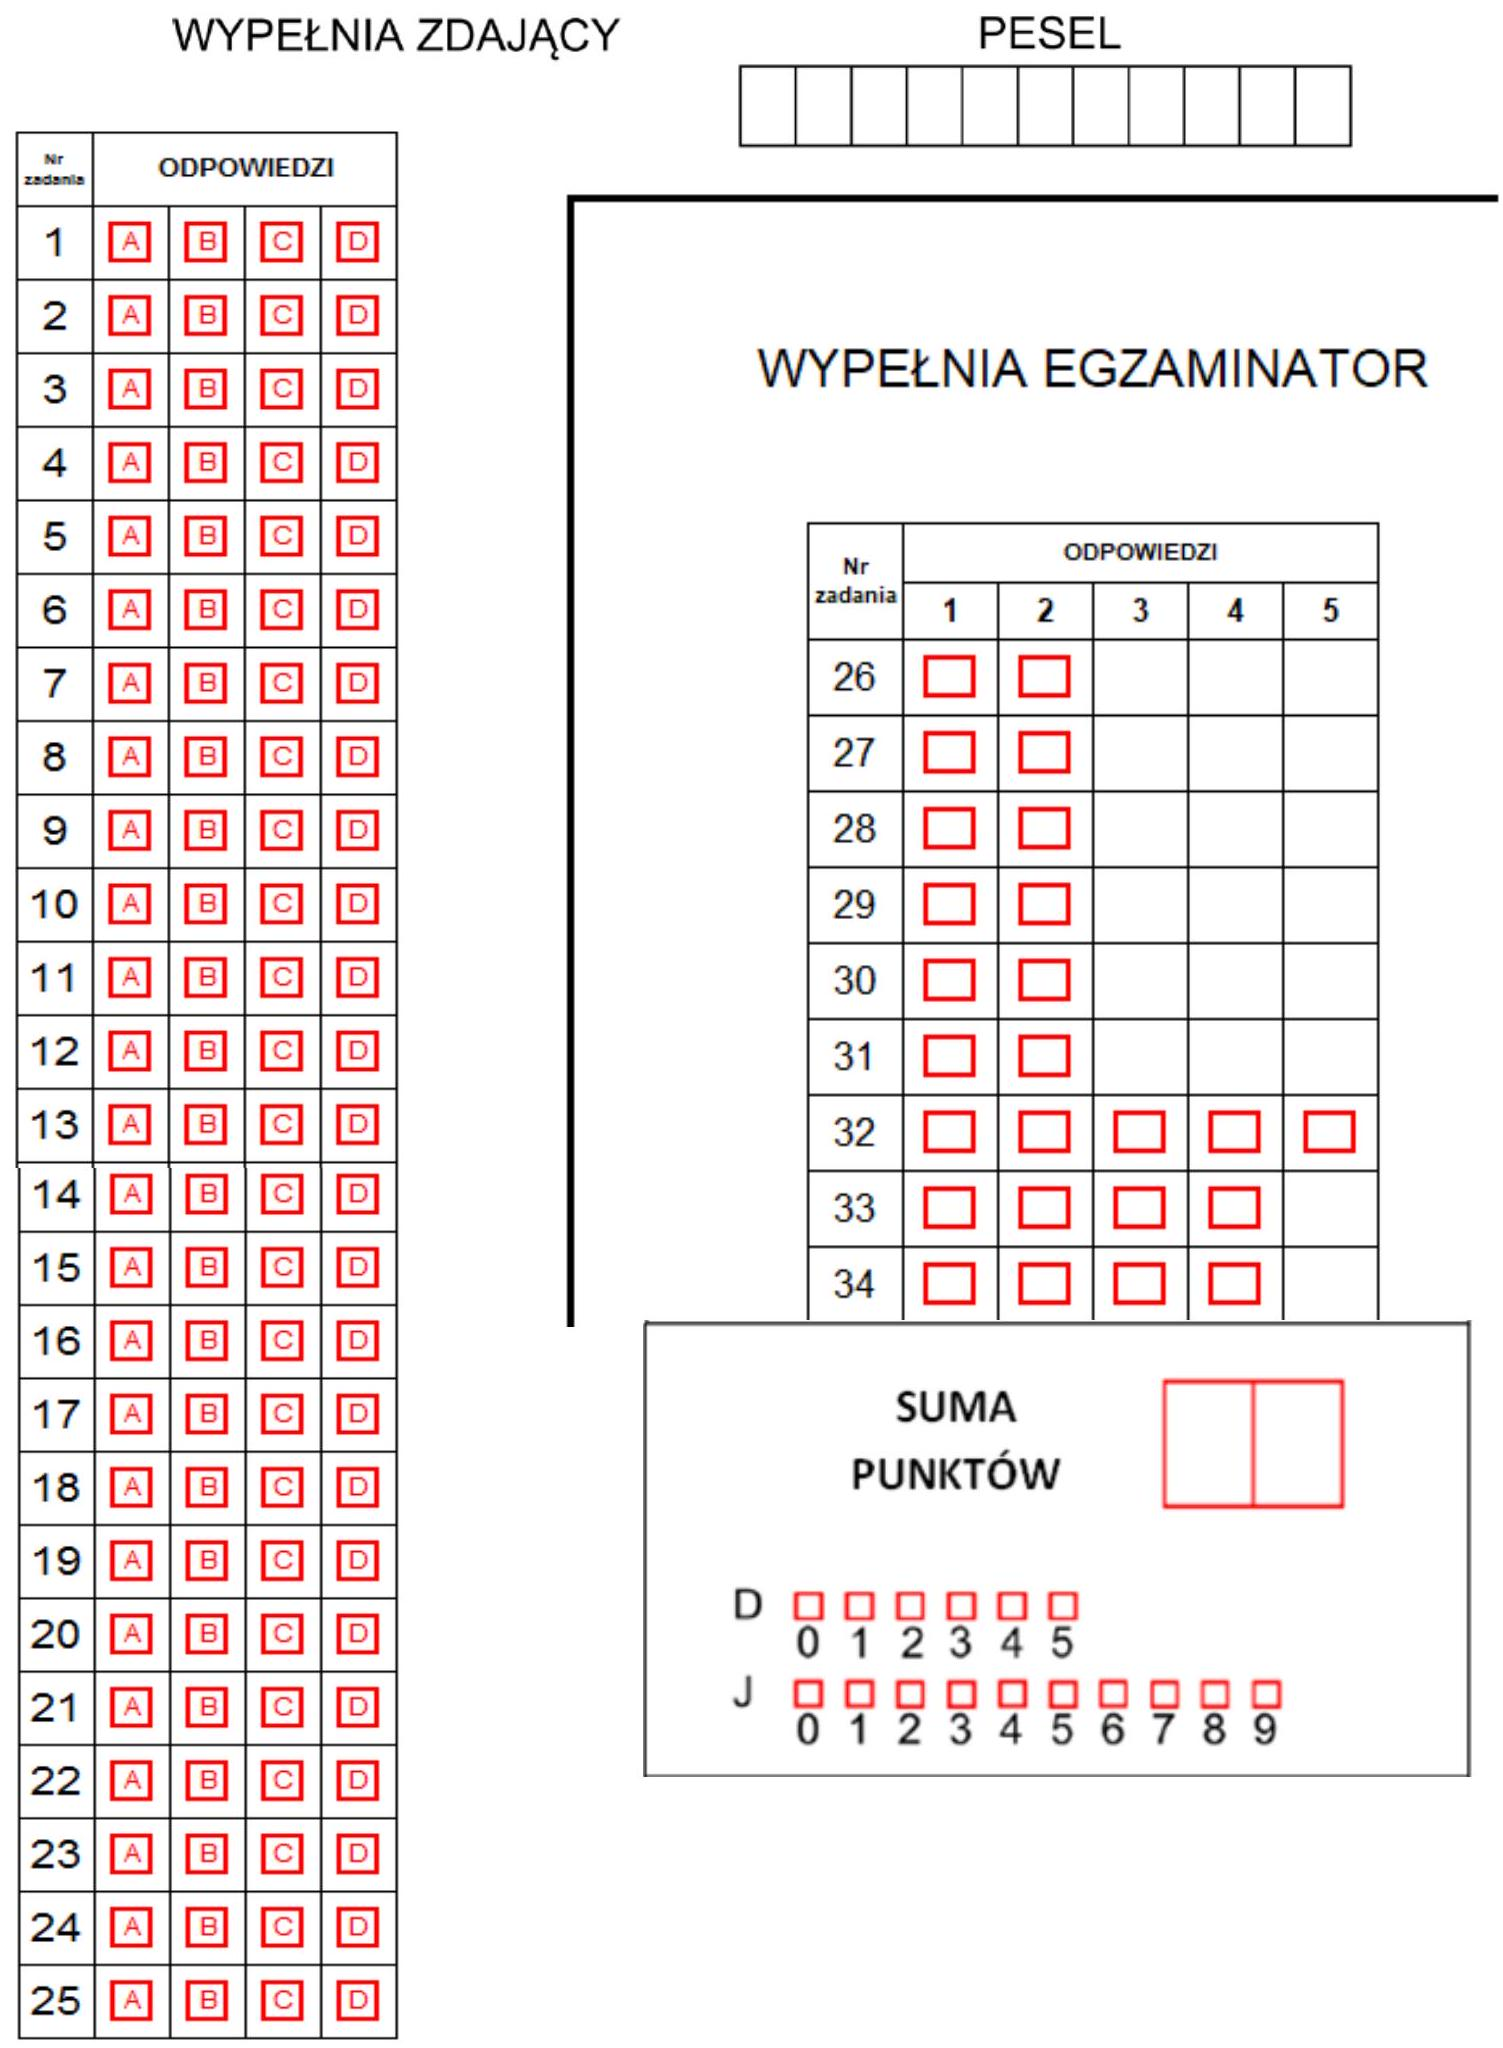
\includegraphics[max width=\textwidth]{2024_11_21_ba65d61981011633d840g-20}
\end{center}


\end{document}